\section{Аналитическая часть}
В данном разделе описываются причины возникновения шумов в изображениях. 
Рассматриваются алгоритмы определения наличия шума на фотографиях. 
Даётся описание существующих методов удаления шумов из картинки, классификации существующих алгоритмов и критериев их сравнения.

\subsection{Причины появления шумов в изображениях}
Шум -- дефект изображения, в основе которого лежит эффект появления на фотографии пикселей случайного цвета и яркости по всему изображению \cite{shum}. 

Причины возникновения такого эффекта делятся на два типа: естественные и искусственные.
Основных источником естественных помех на изображениях является фотосенсор \cite{shum}.
Существует несколько физических объяснений появления шума на изображении \cite{causes}:
\begin{enumerate}
	\item При дефектах потенциального барьера происходит утечка заряда. В этом случае шум на изображениях проявляется в виде тёмных точек на светлом фоне.
	\item При подаче потенциала на электрод может возникнуть темновой ток, который отображается на картинке в виде светлых точек на тёмном фоне. Основная причина возникновения темнового тока — это примеси в кремниевой пластине или повреждение кристаллической решётки кремния. 
	\item Взаимодействие фотонов света с атомами фотодиодов сенсора несёт случайный характер, нельзя точно описать, какие квантовые эффекты при этом возникают.
	\item При производстве фотоаппаратов случается брак, и некоторые пиксели являются дефектными. 
\end{enumerate}

Также шум на изображениях может быть вызван умышленным вмешательством человека или состязательной атакой. 
Состязательная атака – это манипуляция обучающими данными, архитектурой модели или манипулирование тестовыми данными таким
образом, что это приведёт к неправильному выходу из модели машинного обучения \cite{impact}.

Одним из способов такой атаки является изменения на картине некоторых пикселей до такого состояния, что алгоритмы анализа изображения перестают выдавать адекватный результат.


\subsection{Классификация шумов}
Существует несколько основных типов шумов, возникающих на фотографиях \cite{filterTechincs}.
От точного определения характеристики шума зависит то, какой метод требуется выбрать для автоматического определения дефектных пикселей на изображении и последующего его устранения.

\subsubsection{Гауссов шум}
Так как квантовым процессам свойственна случайность, то такие процессы можно отнести к Гауссовым, следовательно, они обладают следующим свойством: распределение суммы независимых случайных величин сходится к нормальному, вне зависимости от характера распределения слагаемых \cite{inproceedings}.

Пусть $I$ -- интенсивность изначального пикселя, а $\nu$ -- интенсивность шума, распределённая по нормальному распределению. 
Тогда интенсивность загрязнённого пикселя можно представить по формуле \ref{gauss} \cite{filterTechincs}: 
\begin{equation}
	\label{gauss}
I_f = I + \nu,  \nu \sim N(0, \sigma^2)
\end{equation}


Вид гауссова шума представлен на рисунке \ref{fig::gaussSh}
\FloatBarrier
\begin{figure}[h]	
	\begin{center}
		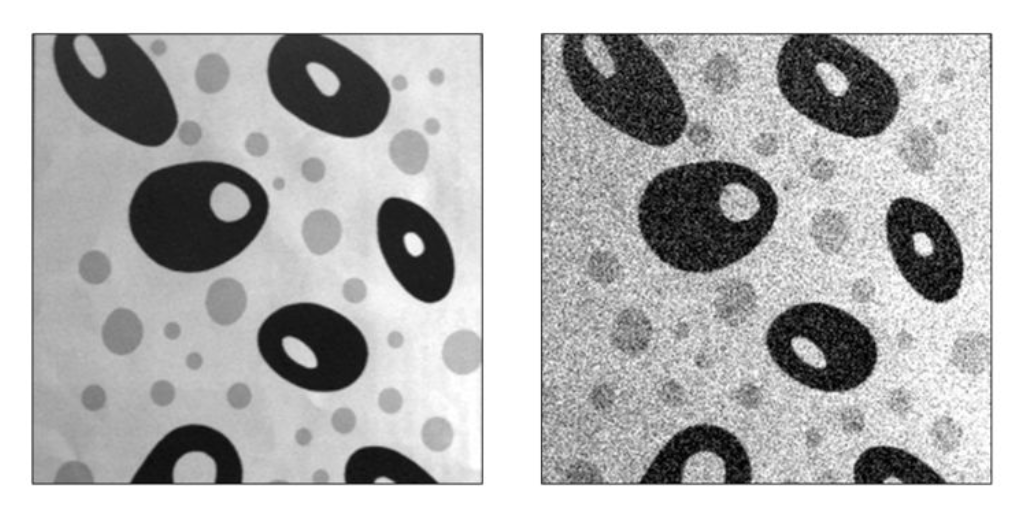
\includegraphics[width=\linewidth]{inc/png/gaussShum.png}
	\end{center}
	\captionsetup{justification=centering}
	\caption{Вид гауссова шума}
	\label{fig::gaussSh}
\end{figure}
\FloatBarrier

Именно этот вид шумов на практике встречается чаще всего. 

\subsubsection{Шум соли и перца}
Шум соли и перца проявляется в том, что на изображениях в случайных местах появляются чёрные и белые пиксели \cite{moments}.
Основной причиной их возникновения является темновой ток и утечка заряда в фотосенсоре, а также наличие пикселей с дефектами \cite{shum}.

Пусть $S$ -- исходное изображение, а $i, j$ -- координаты пикселя. 
Тогда математически описать появление такого шума можно по формуле \ref{saltProbe}: 
\begin{equation}
	\label{saltProbe}
	P(S_{i, j} = 1) = p
\end{equation}

Вид шума соли и перца представлен на рисунке \ref{fig::salt}
\FloatBarrier
\begin{figure}[h]	
	\begin{center}
		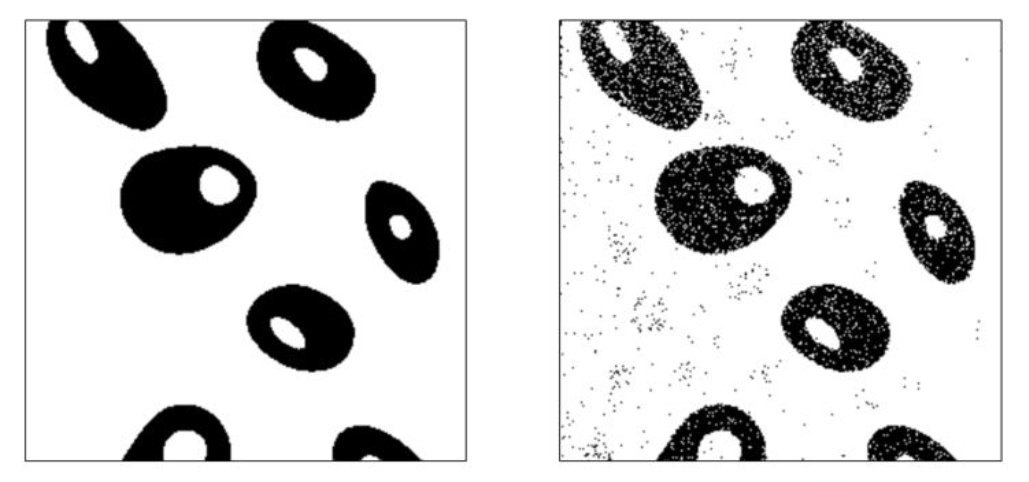
\includegraphics[width=\linewidth]{inc/png/salt.png}
	\end{center}
	\captionsetup{justification=centering}
	\caption{Общая схема работы всех алгоритмов}
	\label{fig::salt}
\end{figure}
\FloatBarrier

Основным методом борьбы с таким видом шумов является медианный фильтр.

\subsubsection{Спекл-шум}
Спекл-шум часто встречается в медицинских методах визуализации, которые основаны на ультразвуке и лазерных технологиях: КТ, ОКТ.
Сложность борьбы с такими помехами состоит в том, вероятность их возникновения описывается не нормальным распределением, а другими, например Гамма-распределением или распределением Релея.

Пусть $I$ -- интенсивность изначального пикселя, а $\nu$ -- интенсивность шума, распределённая по нормальному распределению. 
Тогда интенсивность загрязнённого пикселя можно представить по формуле \ref{spekl}: 
\begin{equation}
	\label{spekl}
	I_f = I * \nu
\end{equation}

Таким образом, влияние спекл-шума может быть значительным, а линейные методы решения таких задач не подходят для того, что исключить шумы из исходного изображения.

\subsection{Существующие методы обнаружения и устранения шумов}
Шумы искажают исходную картинку и портят её качество так, что это способен распознать человеческий глаз.
Однако могут возникнуть трудности в обнаружении помех, поскольку они трудно различимы при совпадении цвета фона и цвета пиксела, например, светлые точки будут плохо заметны на ярком фоне.

Было разработано несколько алгоритмов, которые производят бинарную классификацию пикселей и определяют, какие из них можно идентифицировать как шумы и затем их устранить.

В качестве классификации алгоритмы можно разделить на два типа:
\begin{enumerate}
	\item \textbf{Изотропная фильтрация} -- такие методы устраняют помехи, но не учитывают детали пикселя и увеличивают размытость.
	\item \textbf{Анизотропная фильтрация} -- алгоритмы устраняют эффекты сглаживания, уменьшают размытость и сохраняют детали пикселя, устраняя при этом непосредственно шум из изображения.
\end{enumerate}


\subsubsection{Общий алгоритм работы фильтров}
Алгоритмы, анализирующие наличие шумов в изображениях, имеют дело с различными характеристиками одного пикселя.
Например, цвет пикселя можно разбить на три составляющие -- синюю, красную и зелёную. 

В таком случае метод работает с каждой из составляющих пикселя, вычисляя новое значение для каждой характеристики.
Результат работы в этом случае является объединением подсчётов по всем характеристикам.

Общая схема работы алгоритмов представлена на рисунке \ref{fig::allAlgs}:
\FloatBarrier
 \begin{figure}[h]	
 	\begin{center}
 		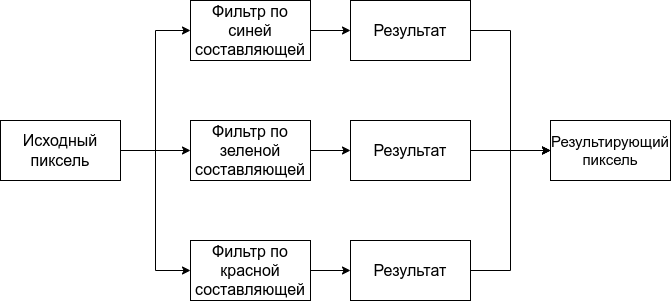
\includegraphics[width=\linewidth]{inc/png/allAlgs.png}
 	\end{center}
 	\captionsetup{justification=centering}
 	\caption{Общая схема работы всех алгоритмов}
 	\label{fig::allAlgs}
 \end{figure}
\FloatBarrier

Каждый из фильтров, перечисленный ниже, работает с каждым из параметров пикселя одинаково, поэтому для корректной работы алгоритмов требуется вычислить значение каждого свойства для результирующего пиксела.

\subsubsection{Медианный фильтр}
Под медианным фильтром понимается семейство однотипных алгоритмов, относящихся к классу нелинейных фильтров.

Метод работает в цикле с каждым пикселем изображения. 
В окрестности каждого пикселя находится восемь соседних, каждый обладает собственными свойствами. 
На рисунке \ref{fig::grid} изображена сетка, с которой работает алгоритм:

\FloatBarrier
\begin{figure}[h]	
	\begin{center}
		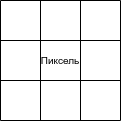
\includegraphics[]{inc/png/grid.png}
	\end{center}
	\captionsetup{justification=centering}
	\caption{Рассматриваемая сетка пикселей при работе алгоритма}
	\label{fig::grid}
\end{figure}
\FloatBarrier
\newpage

Пусть $C_{i, j}$ -- один из параметров рассматриваемого пикселя, а $\Omega$ -- все пиксели сетки.
Алгоритм подсчитывает медиану от такого же параметра соседних клеток и заменяет параметр пикселя на значение этой медианы.
Итоговое значение можно посчитать по формуле \ref{median}: 
\begin{equation}
	\label{median}
	C_{i, j} = median(\Omega_i) 
\end{equation}

Схема работы алгоритма изображена на рисунке \ref{fig::median}:
\FloatBarrier
\begin{figure}[h]	
	\begin{center}
		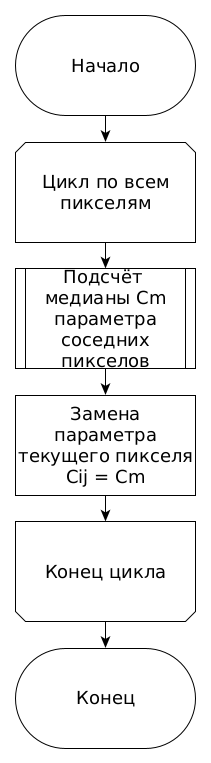
\includegraphics[height=15cm]{inc/png/median.png}
	\end{center}
	\captionsetup{justification=centering}
	\caption{Схема работы алгоритма медианного фильтра}
	\label{fig::median}
\end{figure}
\FloatBarrier

К преимуществам данного метода можно отнести то, что он применяется к любым типам шумов, появившимся в изображении.
Из недостатков -- алгоритм может убрать значительные детали из изображения, посчитав их за шум. 

Медианный фильтр используется в алгоритмах ПО компании Kodak.


\subsubsection{Гауссовский фильтр}
Работа алгоритма гауссовского фильтра также зависит от значений свойств пикселей в сетке, рассмотренной на рисунке \ref{fig::grid}.

В этом случае для каждого соседнего рассчитывается вес, с которым он влияет на новое значение рассматриваемого пикселя. 
Пусть $d$ -- расстояние до центрального пикселя сетки, $\sigma$ -- стандартное отклонение, подсчитанное для всех значений определённого параметра текущей сетки.
Тогда вес $w$ пикселя рассчитывается по формуле \ref{weight}:
\begin{equation}
	\label{weight}
	w_{ij} = \exp(\frac{-d^2}{2\sigma^2})
\end{equation}

Подсчитав вес для каждого пикселя в сетки, можно рассчитать новое значение свойства рассматриваемого пикселя по формуле \ref{gauss::final}:
\begin{equation}
	\label{gauss::final}
	p_i = \frac{1}{\sum_{j \in \Omega}^{} w_{ij}} * \sum_{j \in \Omega}^{} w_{ij} * p_j 
\end{equation}

Схема алгоритма гауссовского фильтра представлена на рисунке \ref{fig::gauss}:
\FloatBarrier
\begin{figure}[h]	
	\begin{center}
		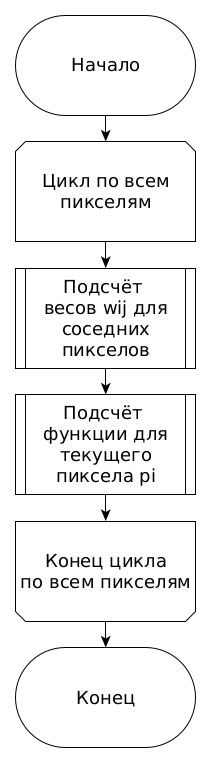
\includegraphics[height=15cm]{inc/png/gauss.png}
	\end{center}
	\captionsetup{justification=centering}
	\caption{Схема работы алгоритма гауссовского фильтра}
	\label{fig::gauss}
\end{figure}
\FloatBarrier

\subsubsection{Двухсторонняя фильтрация}
Алгоритм двухсторонней фильтрации является улучшением метода Гауссовского фильтра.

Для каждого пикселя сетки соседних пикселей используется сразу два веса: один аналогичный параметру из исходного алгоритма, а второй отвечает за анизотропную составляющую. 
В методе рассчитывается разница в определённой компоненте между соседними пикселями.
Если она получилось большой, то это означает, что пиксель содержит какие-то важные детали по изображению, соответственно, фильтрация приведёт к минимальным изменениям фотографии.
Чем меньше разница между соседними пикселями, тем большим будет эффект от фильтрации на рассматриваемой сетке.

Расчёт веса $w_s$, отвечающего за изотропную составляющую, происходит по формуле \ref{weight}. 
Коэффициент, регулирующий анизотропные свойства фильтрации, рассчитывается по формуле \ref{weight2}:
\begin{equation}
	\label{weight2}
	w_{r} = \exp(\frac{-|p_i - p_j|}{2\sigma^2})
\end{equation}

В таком случае результат работы некоторого пикселя можно посчитать по формуле \ref{bilateral}:
\begin{equation}
	\label{bilateral}
	p_i = \frac{1}{\sum_{j \in \Omega}^{} w_{s}w_{r}} * \sum_{j \in \Omega}^{} w_{s}w_{r}p_j 
\end{equation}

Схема работы алгоритма двухсторонней фильтрации представлена на рисунке \ref{fig::bilateral}:
\FloatBarrier
\begin{figure}[h]	
	\begin{center}
		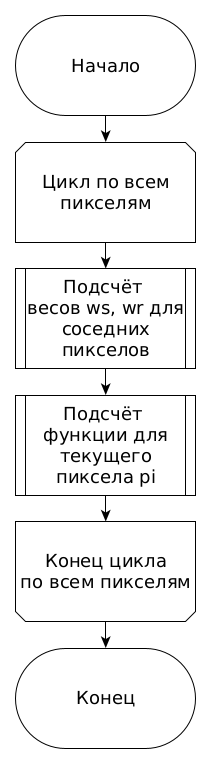
\includegraphics[height=12cm]{inc/png/bilateral.png}
	\end{center}
	\captionsetup{justification=centering}
	\caption{Схема работы алгоритма двухсторонней фильтрации}
	\label{fig::bilateral}
\end{figure}
\FloatBarrier

\subsubsection{Алгоритм Цзяньвэй}
Этот алгоритм был описан в 2014 году индонезийским учёным Ван Цзяньвэй \cite{color_image}
Алгоритм позволяет эффективно убирать шумы соли и перца даже в случае сильной загрязнённости изображения.
Метод предполагает, что для каждого пикселя помехи будут удалены по всем цветовым составляющим.

Процедура заключается в обходе всех пикселей фотографии в заданном порядке и определении того, соответствуют ли значения пикселей функции плотности вероятности импульсного шума или нет. 
Если пиксель на первом классифицируется как шум, то подсчитывается количество импульсного шума в маске определенной формы. 
Если это число меньше чем заданный порог, то пиксель рассматривается как возможный шум. 
Результатом операции маски является замена значения пикселя.
В противном случае это не рассматривается как шум, значение пикселя остается неизменным.

Схема алгоритма Цзяньвэй представлена на рисунке \ref{fig::china}
\FloatBarrier
\begin{figure}[h]	
	\begin{center}
		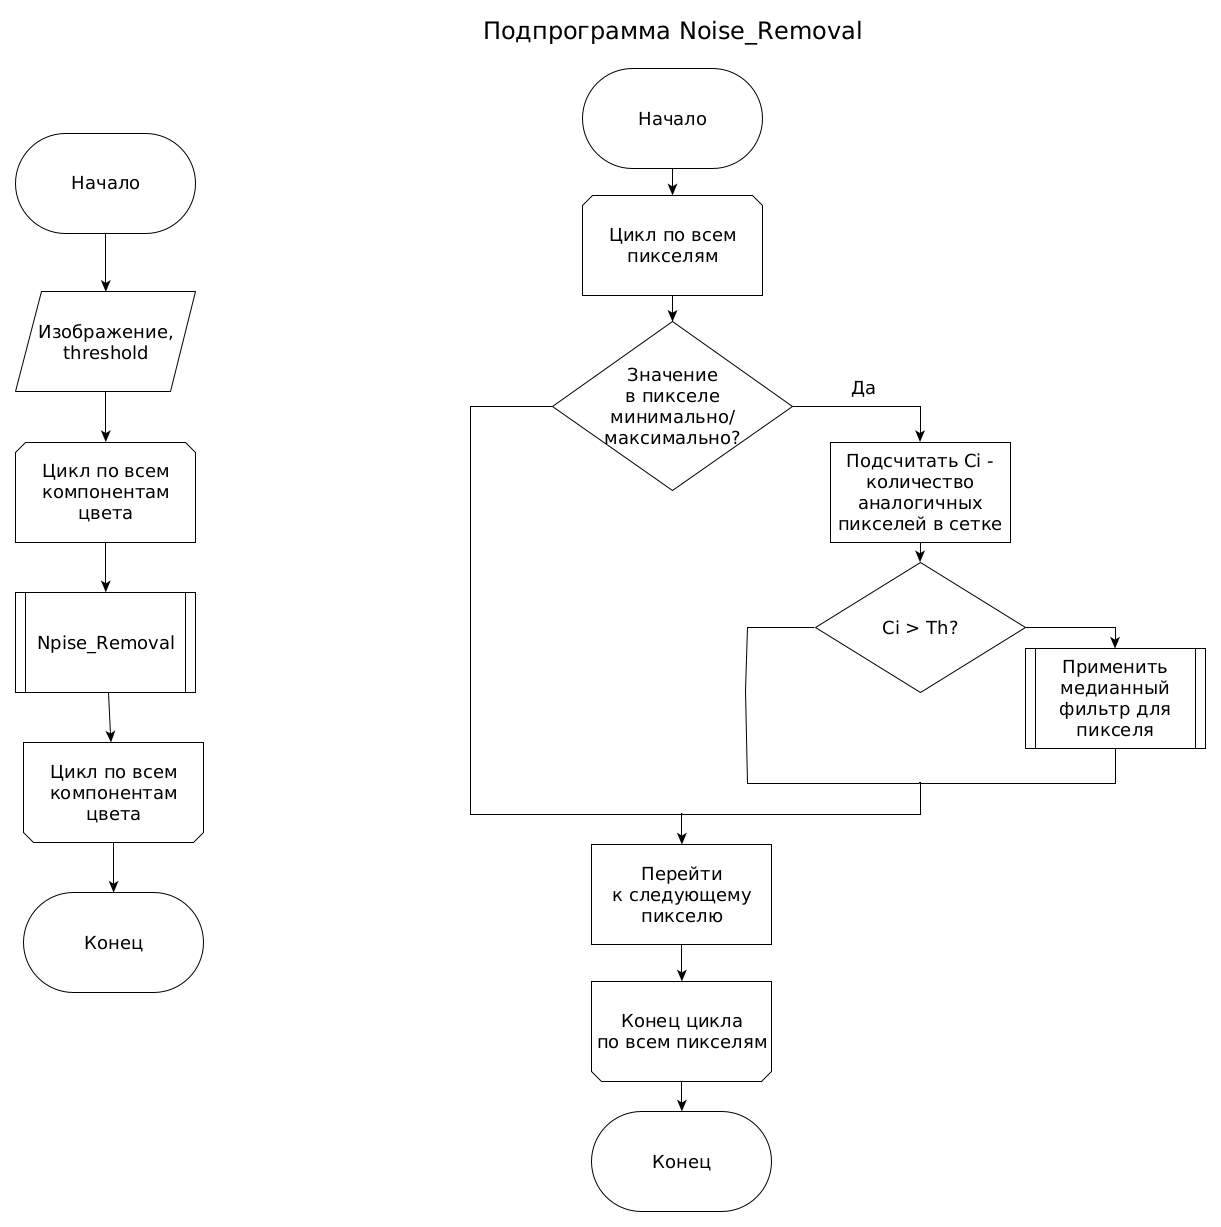
\includegraphics[height=14cm]{inc/png/china.png}
	\end{center}
	\captionsetup{justification=centering}
	\caption{Схема работы алгоритма Цзяньвэй}
	\label{fig::china}
\end{figure}
\FloatBarrier
